\documentclass[a4paper, 12pt]{article}

\usepackage[a4paper, margin=2.5cm, top=2.5cm, bottom=2.0cm]{geometry} % proper margins
\usepackage{amsmath, amssymb} % extended math environment and symbols
\usepackage[us,24hr]{datetime} % `us' makes \today behave as usual in TeX/LaTeX
\usepackage{fancyhdr}
\usepackage[T1]{fontenc} % handling umlauts etc in output
\usepackage{glossaries} % abbreviations
\usepackage{graphicx} % figures
\usepackage[utf8]{inputenc} % handling umlauts etc in input
\usepackage{listings} % code examples
\usepackage{palatino} % main font
\usepackage{siunitx} % units
\DeclareSIUnit \parsec {pc}
\usepackage[dvipsnames]{xcolor}
\usepackage[
unicode,
colorlinks=true,
urlcolor=NavyBlue,
linkcolor=NavyBlue,
citecolor=NavyBlue
]{hyperref}
% comment this out if you would like to remove the 'Version' timestamp in the header of page 1
% \fancypagestyle{plain}{
% \fancyhf{}
% \rhead{\footnotesize Version {\ddmmyyyydate\today} at \currenttime}
% \renewcommand{\headrulewidth}{0pt}}
% example for how to declare an abbreviation using the glossaries package
\newacronym{rmse}{RMSE}{root-mean-square error}
\newacronym{mse}{MSE}{mean squared error}
\newacronym{mcmc}{MCMC}{Markov chain Monte Carlo}
% example for how to declare non-standard units using the siunitx package
\DeclareSIUnit{\atom}{atom}

\usepackage[backend=biber, style=ieee]{biblatex}
\setlength\bibitemsep{0.5\baselineskip}
\addbibresource{citations.bib}

\parskip 10pt
\parindent 0pt

\usepackage{float}

\begin{document}
% This sets the default language for the listings package.
\lstset{language=Python}
\title{
\sffamily
\vspace{-1.7cm}
{\huge\textbf{Project 1 -- Cosmological Models}} \\[-0.4cm]
}
\author{
    \vspace{-0.4cm}
    \begin{minipage}[t]{0.45\textwidth}
\centering
Linus Brink\\
\href{mailto:brinkl@chalmers.se}{brinkl@chalmers.se}
\end{minipage}%
\hfill
\begin{minipage}[t]{0.45\textwidth}
\centering
Oscar Stommendal\\
\href{mailto:oscarsto@chalmers.se}{oscarsto@chalmers.se}
\end{minipage}
}
\date{\today}
\maketitle
% \begin{center}
%     \textbf{Abstract}
% \end{center}
\vspace{-1.5cm}
\section{Introduction}
Understanding the universe is one of the most fascinating challenges in science. Cosmology, the study of the universe as a whole, seeks to solve the mysteries of its origin, evolution, and fate. In this project, we explore cosmological models using observational supernovae data to extract key cosmological parameters such as the Hubble constant $H_0$ and the deceleration parameter $q_0$. We also investigate different cosmological models and assess their fit to the data.
\vspace{-0.5cm}
\section{Theory}
Type Ia Supernovae are considered standardizable candles in cosmology due to their consistent brightness \cite{projpdf}. By measuring their apparent brightness and redshift $z$, we can infer distances and probe the expansion history of the universe. The distance modulus $\mu$ relates the apparent magnitude $m$ and absolute magnitude $M$ of a supernova,
\begin{equation}\label{d_L}
\mu = m - M = 5 \log_{10}(d_\mathrm{L}) + 25,
\end{equation}
where $d_\mathrm{L}$ is the luminosity distance in Mpc. In a flat universe, $d_\mathrm{L}$ is given by
\begin{equation}
    d_\mathrm{L}(z) = c(1 + z) \int_{0}^{z} \frac{dz^\prime}{H(z^\prime)},
\end{equation}
where $H$ is the Hubble parameter and $c$ the speed of light. In this case, the Friedmann equation reduces to $1 = \Omega_M + \Omega_\Lambda$, where $\Omega_M$ and $\Omega_\Lambda$ are the matter and dark energy density parameters. By normalizing these with present values (subscript 0), one can get the reduced version of the so called $\Lambda$CDM cosmology
\begin{equation}\label{lCDM}
    H(z) = H_0 \sqrt{\Omega_{\mathrm{M},0}(1+z)^3 + \Omega_{\Lambda,0}} \equiv H_0\,E(z)^{1/2}.
\end{equation}

For $z << 1$ (generally accepted to be $z < 0.5$), Taylor expansion gives of Eq. \ref{lCDM} leads to $E(z) \approx 1 + 2z\,(q_0 + 1)$, where $q_0 = (\Omega_{M,0} - 2\Omega_{\Lambda,0})/2$ is called the deceleration parameter, showing if the Universal expansion is decelerating ($q_0>0$) or accelerating ($q_0<0$). In the small-$z$ domain, $d_L$ can also be rewritten as 
\begin{equation}\label{small_z}
    d_L(z) = c(1+z)\int_{0}^{z}\frac{dz'}{H(z')} \approx \frac{c}{H_0}\left( z + \frac{1}{2}(1-q_0)z^2 + \dots \right).
\end{equation}

Other cosmologies can also be explored within the flat Universe. An extension to the flat $\Lambda$CDM is the so-called wCDM cosmology, which has the extra dark-energy equation-of-state parameter w, leading to a Hubble parameter corresponding to
\begin{equation}\label{wCDM}
    E(z) = \Omega_{\mathrm{M},0}(1+z)^3 + \Omega_{\Lambda,0}(1+z)^{3(1+w)}.
\end{equation}
\vspace{-1.2cm}
\section{Methodology}
The first task was to infer values on the Hubble constant $H_0$ and deceleration parameter $q_0$ from provided supernova data using a Bayesian framework. The data consisted of redshift values $z$, observed distance moduli $\mu_{\text{obs}}$, and their associated uncertainties $\sigma_{\mu}$ for 833 Type Ia supernovae \cite{SCPwebsite}. Accordingly, log prior, log likelihood, and log posterior functions were defined. The prior distributions for $H_0$ and $q_0$ were chosen to be uniform within bounds based on prior knowledge from cosmological observations. We used $H_0 \in [30, 100]\,\si{\kilo\metre\per\second\per\mega\parsec}$ and $q_0 \in [-2, 2]$. For the unknown error variance parameter $s^2$, we used an inverse gamma prior with shape set to 1 and scale set to 1.

The likelihood function was constructed assuming Gaussian errors on the observed $\mu$,
\begin{equation}
    \ln \mathcal{L}(\mu_{\text{obs}} | H_0, q_0, s^2) = -\frac{1}{2} \sum_{i} \left[ \frac{(\mu_{\text{obs},i} - \mu_{\text{model},i})^2}{\sigma_{\mu,i}^2s^2} + \ln(2\pi\sigma_{\mu,i}^2s^2) \right],
\end{equation}
where $\mu_{\text{model},i}$ is the model-predicted distance modulus from equation \ref{d_L} for the $i$-th supernova given parameters $H_0$ and $q_0$, and $\sigma_{\mu,i}$ is the observational uncertainty. To calculate $d_L$ using parameters $H_0$ and $q_0$, Eq. \ref{small_z} up to second order was used, as we only considered supernovae with $z < 0.5$. Following Bayes' theorem, the log posterior is then given by the sum of the log prior and log likelihood.

To sample the posterior distribution, Markov Chain Monte Carlo (MCMC) was employed using the \texttt{emcee} package \cite{emcee}. 100 walkers were initialized randomly within the prior bounds and run for 6000 iterations, discarding the first 1000 iterations as burn-in. Convergence was assessed by visually inspecting trace plots. After sampling, posterior distributions for $H_0$, $q_0$, and $s^2$, were analyzed. Corner plots using the \texttt{corner} package were created to visualize the joint and marginal posterior distributions of the parameters \cite{corner}. In addition to the posterior analysis, posterior predictive checks were performed to assess the model fit. Using the posterior samples and Eq. \ref{d_L} and \ref{small_z}, predicted distance moduli $\mu_{\text{model}}$ were generated across the original range of redshift values $z \in [0.1, 1.5]$, i.e., not only for small $z$, and compared to the observed data. %The median of the predicted distance moduli was plotted alongside the observed data in order to visually evaluate the model's performance.

The second part of the project focused on comparing the $\Lambda$CDM and wCDM cosmological models defined by the expressions for $H(z)$ in Eq. \ref{lCDM} and \ref{wCDM}. Due to the increased complexity when considering the full redshift range in Eq. \ref{small_z}, the models were compared using AIC and BIC scores. The log-likelihood function was modified to account for the whole redshift range, using the \texttt{scipy} package to perform the necessary numerical integration for $d_\mathrm{L}(z)$ in Eq. \ref{small_z} \cite{2020SciPy-NMeth}. The same package was used to optimize the log-likelihood function for both models, yielding maximum log-likelihood estimates for the parameters. The AIC and BIC scores were then calculated using the formulas
\begin{align}
    \text{AIC} &= 2\ln(\mathcal{L}^\star) - 2k \label{eq_AIC}\\
    \text{BIC} &= 2\ln(\mathcal{L}^\star) - k \ln(N) \label{eq_BIC},
\end{align}
where $k$ is the number of model parameters, $N$ the number of data points, and $\mathcal{L}^\star$ the maximum likelihood value. The model with the higher AIC and BIC scores was considered to have a better balance between fit quality and model complexity. In this case, we assumed that the overall variance was known and equal to the sample variance of the observed distance moduli. From the maximum likelihood estimates, we also found the matter and dark energy density parameters $\Omega_{\mathrm{M},0}$ and $\Omega_{\Lambda,0}$ for both models. 

Finally, MCMC sampling was performed for the $\Lambda$CDM model to obtain the posterior distribution of $\Omega_{\mathrm{M},0}$. The same MCMC setup as before was used, however this time using 10 walkers and 1\,100 iterations due to the increased complexity, discarding the first 100 as burn-in. As above, we also considered the overall variance scale known in this case. For $H_0$, we fixed its value at 70 \si{\kilo\metre\per\second\per\mega\parsec}, and for $\Omega_{\mathrm{M},0}$, we used a uniform prior with values $\Omega_{\mathrm{M},0} \in [0, 1]$. The posterior samples were analyzed to derive credible intervals and visualize the marginal posterior distribution of $\Omega_{M,0}$.
\vspace{-0.5cm}
\section{Results}
Fig.~\ref{fig:corner_plot} shows the joint and marginal posteriors for $H_0$, $q_0$, and $\sigma_\mathrm{sys}^2$, together with corresponding trace panels. The diagonal marginals are close to Gaussian, with posterior medians and 68\% credible intervals $H_0 = 69.79^{+0.42}_{-0.41}\,\mathrm{km\,s^{-1}\,Mpc^{-1}}$, $q_0 = -0.419^{+0.069}_{-0.070}$, and $\sigma_\mathrm{sys}^2 = 0.940^{+0.067}_{-0.062}$. The negative $q_0$ indicates accelerated expansion, and a $\sigma_\mathrm{sys}^{2}$ near unity indicates that the quoted uncertainties require no overall rescaling. The contours reveal a clear negative correlation between $H_0$ and $q_0$ (meaning that as $H_0$ increases, we have a stronger present-day cosmic acceleration, i.e., lower $q_0$) and only weak coupling of $\sigma_\mathrm{sys}^2$ to the other parameters. The trace panels are stationary and show rapid mixing, consistent with adequate burn-in removal and stable sampling.

\begin{figure}[H]
    \centering
    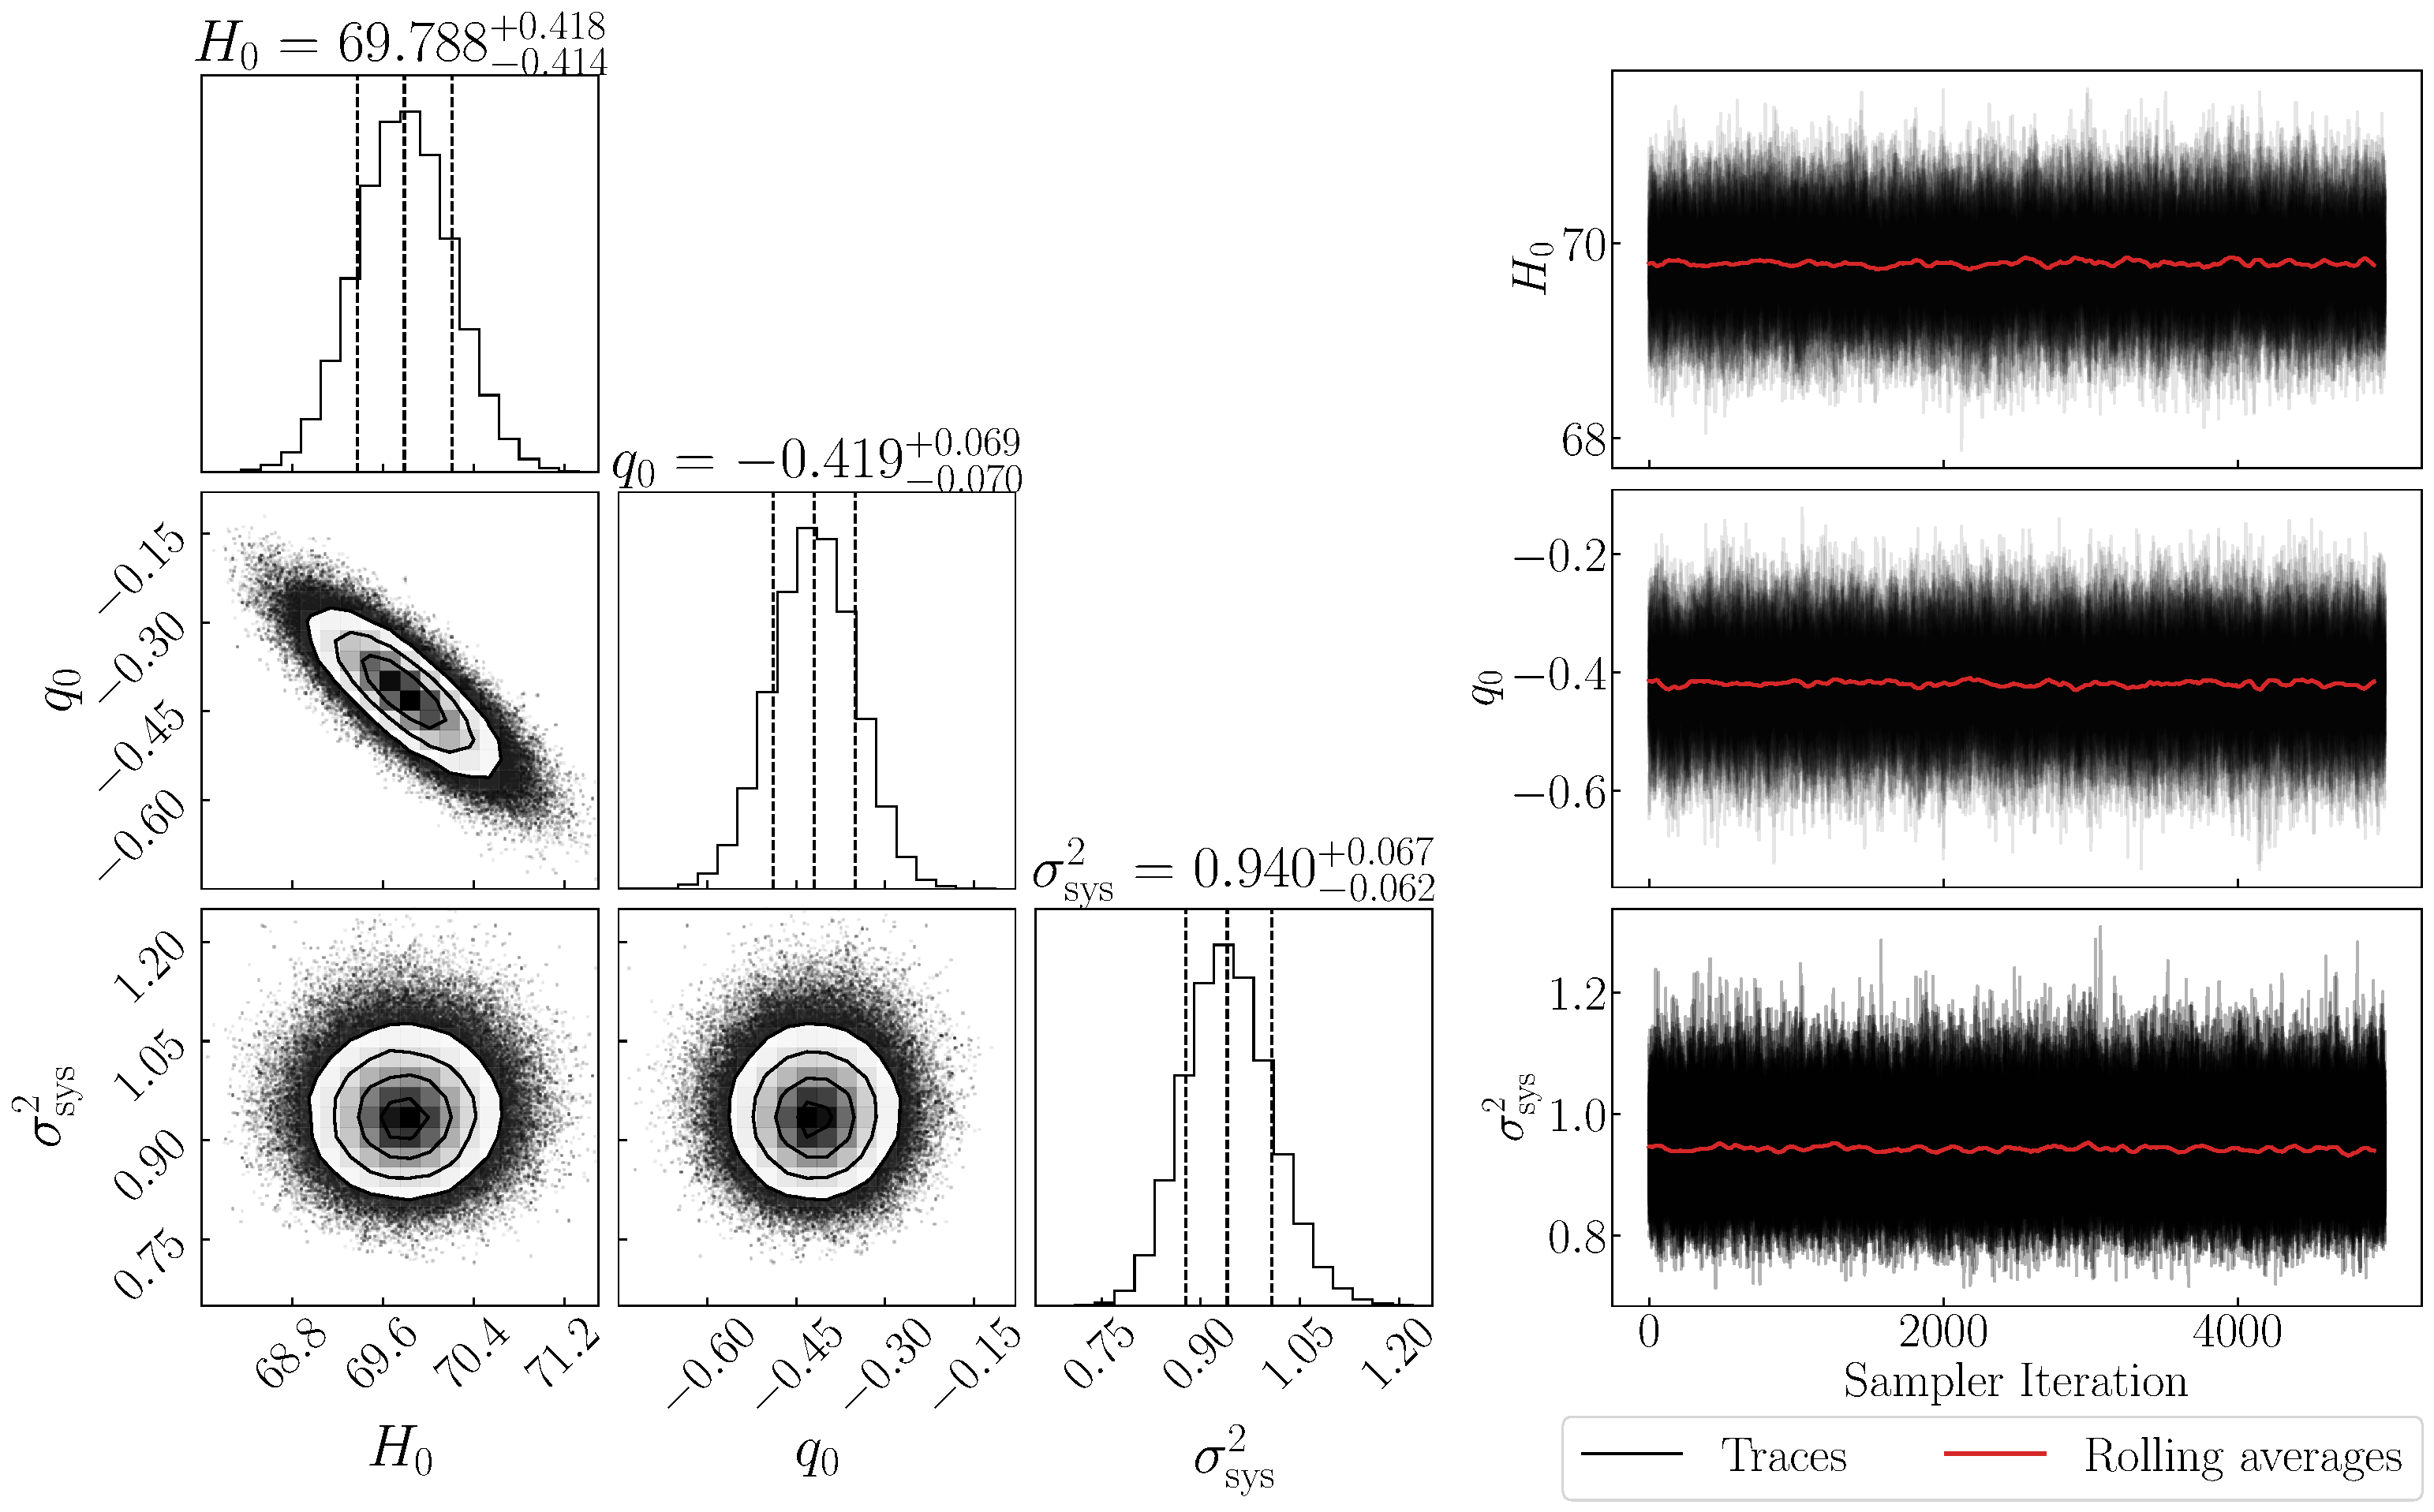
\includegraphics[width=\textwidth, trim={0.2cm 0.1cm 0.2cm 0.1cm}, clip]{figs/post_samples_H0_q0_sigma2.pdf}
    \vspace{-0.1cm}
    \caption{Left: Corner plot showing the posterior distributions and correlations between $H_0$, $q_0$, and $\sigma_{\mathrm{sys}}^2$. The histograms on the diagonal represent the marginal distributions, while the off-diagonal plots show the joint distributions. Right: Trace plots for the MCMC chains of each parameter.}
    \label{fig:corner_plot}
\end{figure}
\newpage
Fig.~\ref{fig:posterior_predictive} displays the Hubble diagram: distance modulus $\mu$ versus redshift $z$ for the supernova data together with the small-$z$ model curve $\mu(z<0.5;H_0,q_0)$ evaluated using the posterior median parameters from Fig.~\ref{fig:corner_plot}. The curve follows the data closely for $z\lesssim 0.5$ and exhibits the gentle upward curvature expected for $q_0<0$. For $z\gtrsim 0.5$ systematic departures between the second-order model and the points become apparent, reflecting the limited validity of the small-$z$ expansion at higher redshift. The vertical scatter of the low-$z$ points about the curve is comparable to the quoted uncertainties, consistent with the inferred variance scale $\sigma_\mathrm{sys}^{2}\simeq 1$.

\begin{figure}[H]
    \centering
    \includegraphics[width=0.6\textwidth]{figs/mu_model_pred.pdf}
    \vspace{-0.4cm}
    \caption{Posterior predictive check showing the observed distance moduli (red points) with error bars and the model median (black line) as a function of redshift $z$.}
    \label{fig:posterior_predictive}
\end{figure}
\vspace{-0.3cm}
Using the full redshift range with $H_0=70\,\mathrm{km\,s^{-1}\,Mpc^{-1}}$ to compare the two flat models, $\Lambda$CDM and wCDM, yields very similar maximum-likelihood estimates ($\Omega_{\mathrm{M},0}\approx 0.28$ and $\Omega_{\Lambda,0}\approx 0.72$), see Table~\ref{tab_IC}. The fitted $w$ is essentially $-1$, making wCDM consistent with $\Lambda$CDM within the precision of this dataset. The AIC and BIC values in Table~\ref{tab_IC} are slightly higher for $\Lambda$CDM, favoring the simpler model. This is consistent with the wCDM fit settling at $w\approx -1$ while introducing an additional parameter.
\vspace{-0.3cm}
\begin{table}[H]
    \centering
    \caption{AIC and BIC scores for the $\Lambda$CDM and wCDM models, along with the maximum likelihood estimates of $H_0$, $\Omega_{\mathrm{M},0}$, $\Omega_{\Lambda,0}$, and $w$.}
    \vspace{0.2cm}
    \begin{tabular}{l|c|c|c|c|c|c}
        \textbf{Model} & \textbf{AIC} & \textbf{BIC} & $\bf{H_0}$ (\si{\kilo\metre\per\second\per\mega\parsec}) & $\bf{\Omega_{M,0}}$ & $\bf{\Omega_{\Lambda,0}}$ & $\bf{w}$ \\ \toprule
        $\Lambda$CDM & 233.5 & 224.8 & 70.0 & 0.278 & 0.722 & -- \\
        wCDM & 231.5 & 218.4 & 70.0 & 0.281 & 0.719 & --1.01 \\ \bottomrule
    \end{tabular}
    \label{tab_IC}
\end{table}
\vspace{-0.3cm}
The marginal posterior for $\Omega_{\mathrm{M},0}$ under flat $\Lambda$CDM (known measurement variances) peaks near the maximum-likelihood value reported in Table~\ref{tab_IC}, providing a consistent central estimate around $\Omega_{\mathrm{M},0}\approx 0.28$. The distribution is tight and symmetric, indicating the full-redshift data constrain $\Omega_{\mathrm{M},0}$ well. The posterior mass lies well away from the boundaries $\Omega_{\mathrm{M},0}=0$ and $1$, and the mode and median are in close agreement with the best-fit value. Sampler traces have clearly converged, indicating adequate mixing and stable estimates.

\begin{figure}[H]
    \centering
    \includegraphics[width=0.99\textwidth]{figs/post_samples_Om_LCDM.png}
    \vspace{-0.4cm}
    \caption{Left: Marginal posterior distribution of $\Omega_{\mathrm{M},0}$ under the $\Lambda$CDM model. The thick dashed line indicate the mean value, while the dotted lines represent 1$\sigma$ credible intervals. Right: Trace plot for the MCMC chain of $\Omega_{\mathrm{M},0}$.}
    \label{fig:Om_marginal_posterior}
\end{figure}
\vspace{-1.2cm}
\section{Discussion}
Earlier measurements place $H_0$ near $70~\mathrm{km\,s^{-1}\,Mpc^{-1}}$ \cite{expvalue_H0} and $q_0$ around $-0.6\pm0.2$ \cite{expvalue_q0}, consistent with the corner-plot estimates. A small-$z$ ($z<0.05$) Hubble-law check by discarding the second order term in Eq. \ref{small_z} gives $H_0 = 68.31 \pm 5.75~\mathrm{km\,s^{-1}\,Mpc^{-1}}$, supporting the distance-modulus calibration and the $H_0$ extraction. Together with $\sigma_\mathrm{sys}^{2}\approx 1$ and the decisively negative $q_0$, this provides robust evidence for acceleration.

The Hubble diagram confirms the small-$z$ approximation’s scope, with good agreement for $z\lesssim 0.5$ and expected drift at higher $z$. A single full-$z$ fit is therefore the natural next step. Using the full luminosity–distance integral with a redshift-aware noise model (intrinsic scatter or Student-$t$, a low-$z$ velocity floor, and propagated systematics) would sharpen $q_0$ by using curvature in $\mu(z)$ and tighten $H_0$ once a distance anchor is included, which should improve inference for both parameters.

Over the full range, the best-fit matter densities are $\Omega_{\mathrm{M},0}=0.278$ for flat $\Lambda$CDM and $0.281$ for flat wCDM, essentially matching the Supernova Cosmology Project values for this dataset ($0.277$ and $0.281$) \cite{Suzuki_omegaM}. This agreement indicates that the distance–redshift model, weighting, and optimizer behave as intended under flatness. AIC and BIC slightly prefer the simpler $\Lambda$CDM. This is consistent with wCDM largely imitating $\Lambda$CDM with one additional parameter, adding complexity without a commensurate gain in fit and increasing overfitting risk. The $\Omega_{\mathrm{M},0}$ posterior places most of its mass well away from the prior bounds (Fig.~\ref{fig:Om_marginal_posterior}), indicating a data-driven constraint rather than a prior-limited one.

The most time went into interpreting the weighting instruction and implementing a global error-scale $\sigma_\mathrm{sys}^{2}$ that multiplies per-supernova variances rather than normalizing by sample size. A subtle point was what $\sigma_\mathrm{sys}^{2}\approx 1$ actually means. It is a uniform rescaling of the quoted variances, so $\sigma_\mathrm{sys}^{2}=1$ does not imply vanishing error, only that no global inflation or deflation is needed. It was reassuring that $\sigma_\mathrm{sys}^{2}$ landed near $1$, that $w$ tended to $-1$, and that $\Omega_{\mathrm{M},0}$ matched the Union2.1 value for this dataset, which together supported that the implementation and weighting behaved as intended.


\printbibliography

\end{document}